\subsection{An Agenda-based Dialog Management Architecture for Spoken Language Systems \cite{Rudnicky1999a}}

This paper proposes a dialog management architecture based on the elements of \emph{handlers}, a \emph{product} and an \emph{agenda}. The goal is to develop a dialog management that can solve two specific problems: 1) providing a coherent coverall structure to interaction that extends beyond the single turn; 2) correctly manage mixed-initiative interaction.

When the paper was written there were two commonly used dialog management approaches: \emph{graph-flow based} systems and \emph{frame-based} systems. Graph-based systems handle the dialog by explicitly enumerating all possible dialog states, as well as allowable transitions between states. However, graph systems have a number of limitations, such as making it difficult for a user to change topic. The frame-based method does not necessarily extend to more complex tasks, for example ones where the goal is to create a complex data object, such as a plan.

The paper first describes a \emph{script-based dialog manager}, before formally introducing the more sophisticated agenda-based architecture. Script in the context simply refers to an explicit sequencing of task-related topics. Each topic is expressed as a form-filling task. In the control strategy, slots are pre-ordered based on their ability to constrain the solution; this ordering provides a default sequence in which the system selects to ask the user about. Figure \ref{fig:R99a-script_based} shows the structure of the Flight Leg topic in the script-based system.

\begin{figure}[h]
  \centering
  % Requires \usepackage{graphicx}
  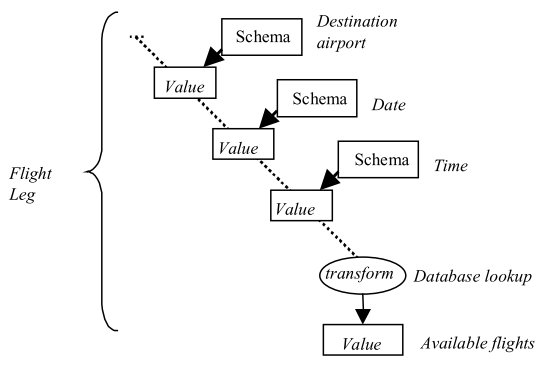
\includegraphics[width=.6\linewidth]{R99a-script_based.png}\\
  \caption{Task-based dialog control in a script-based system.}\label{fig:R99a-script_based}
\end{figure}

The script-based approach still has a number of limitation, such as making it difficult to navigate over the product. So the paper further proposes an \emph{agenda-based} architecture.

The proposed architecture introduces two new data structures: an \emph{agenda} to replace a fixed script, and a \emph{dynamic product} that could evolve over the course of a session. In the agenda-based system, the product is represented as a tree, which reflects the natural hierarchy and order of the information needed. A dynamic product is simply one that can be modified over the course of a session.

Operationally, this means providing a set of operators over tree structures and making these available to the user and to the system. Each node in the product tree corresponds to a handler, which encapsulates computation relevant to a single information item. The agenda is an ordered list of topics, represented by handlers that govern some single item or some collection of information. The agenda specifies the overall ``plan'' for carrying out a task.
The handler on the top of the agenda has the highest priority and represents the focused topic. When a user input comes in, the system calls each handler per their order in the agenda, and each handler will try to interpret the user input and generate the response.

The proposed dialog management architecture is implemented in the \emph{CMU Communicator} system, which handles a complex travel task consisting of air travel, hotels and car reservations. The system uses the \emph{Sphinx II} speech recognizor in a real-time mode and supports barge-in. A top-1 hypothesis is produced by the decoder and parsed by \emph{Phoenix} using a semantic domain-specific grammar. The example dialog presented in the paper shows a number of features of the proposed architecture: the ability to absorb implicit changes of topic on the part of the user, adding to an existing itinerary, and handling explicit topic shifts.
